%\vspace{-.3cm}
\section{\name \Fs} 
\label{sec:stroll-arch}
%\vspace{-.2cm}

 \name provides accessibility for submission, monitoring/control, and output collection of HPC jobs through the execution of \rc and \wc \fs commands. \figref{fig:system-arch} illustrates the architecture of the entire Job execution model driven by \name, and how its various components interact with the targeted HPC frameworks. The architecture involves the following layers:


\begin{figure}[htbp]
  \centering
  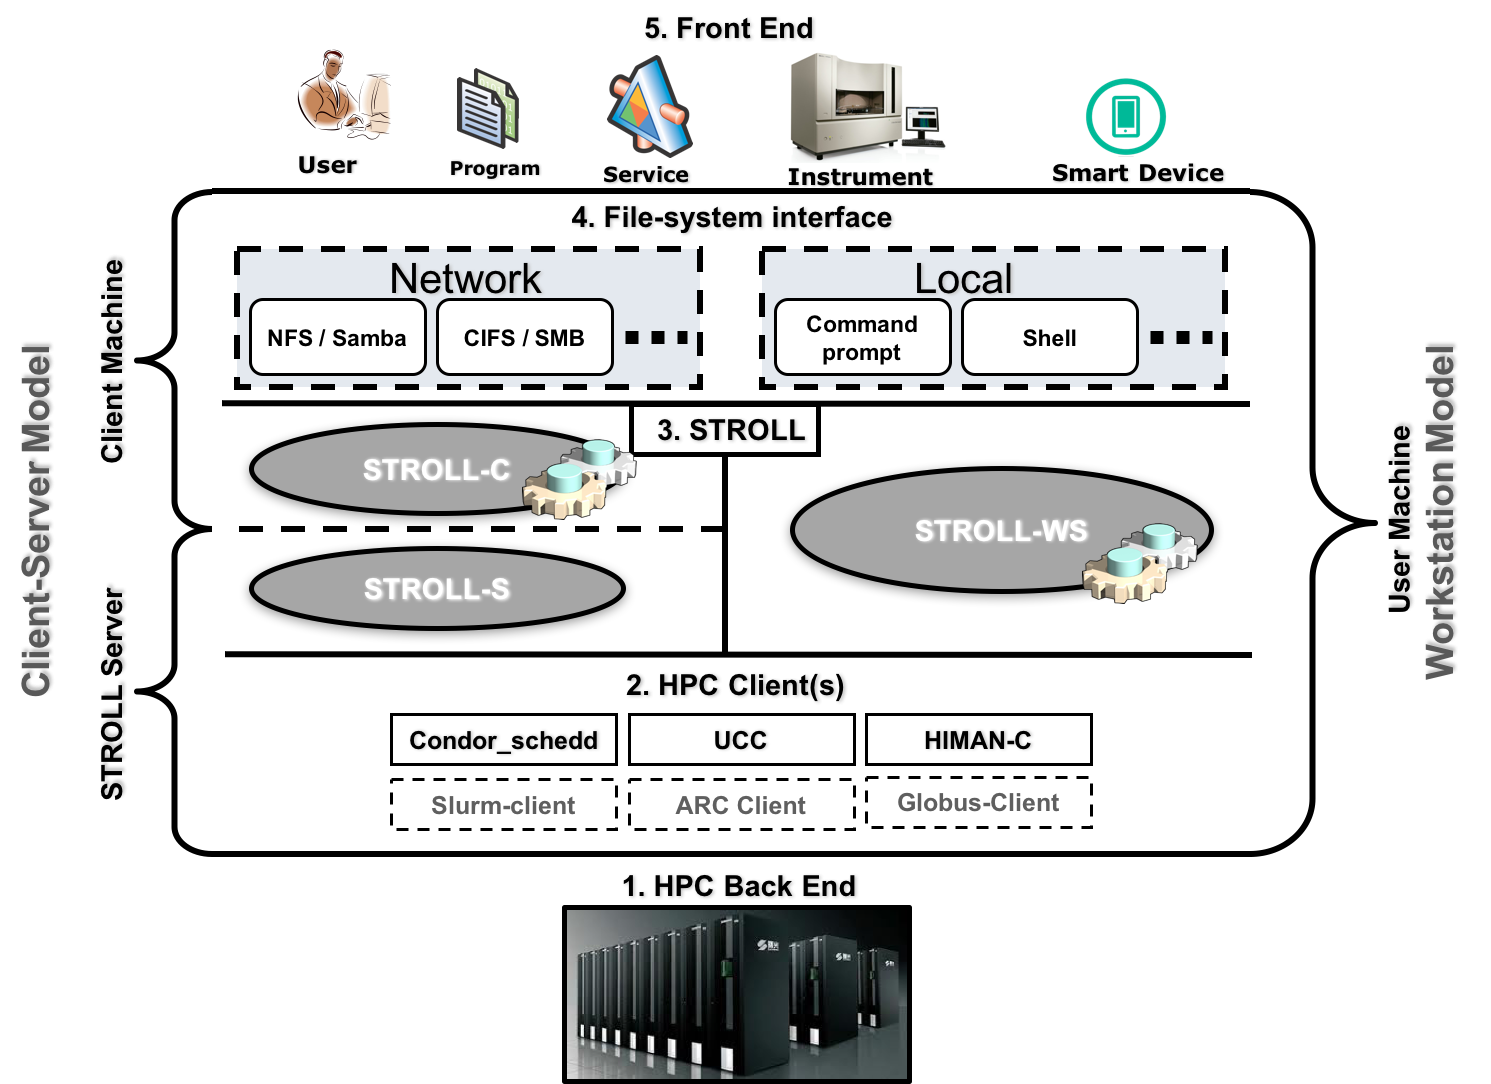
\includegraphics[width=0.5\textwidth]{figures/stroll-arch}                
  \caption{System Architecture}
  \label{fig:system-arch}
\end{figure}

\begin{enumerate}
	\item \textbf{Front-end:} is the front end where job submission is carried out by executing \rc/\wc \fs commands. 
	\item \textbf{File-system interface:} is the interface through which access to \name is done through the execution of \fs commands. This access is supported by any OS through a local \fs interface, e.g. shell and command.com, or remotely, e.g. by sharing the virtual access path and mounting it as a network storage.
	\item \textbf{\name \fs:} is the synthetic \fs which role is to translate \fs commands into a standard job submission script for the cluster and submits it to the target cluster client. \name \fs Layer is either workstation or client-server.
	\item \textbf{HPC Client:} Which includes one or more HPC cluster clients attached to one or more queuing systems. The installed cluster clients are either command line, e.g. $slurm\_client$ for SLURM~\cite{slurm}, $condor\_schedd$ for HTCondor~\cite{condor-paper}, or API based, e.g. HiLA~\cite{hila} for UNICORE~\cite{unicore-paper}, and has to be granted access to existing cluster back end.
	\item \textbf{HPC back-end:} One or more HPC clusters, e.g. HTCondor and UNICORE, could be included as a back end in the setup. To execute job submission/management commands on one of the attached HPC clusters through \name, the users need to be registered in the targeted cluster(s) and granted the associated privileges.
\end{enumerate}

The architecture of \name is depicted in \figref{fig:stroll-arch}, as the server part of layer~3 in \figref{fig:system-arch}, which is a shim layer between the \fs interface and cluster clients. The shim layer is composed of a virtual \fs driver, a command handler, a broker, and a HPC cluster driver. The workstation architecture in \figref{fig:stroll-ws} is described in our main \name paper~\cite{stroll}. The difference between the workstation and the client server architecture is mainly in the \name layer, i.e. layer~3:
\begin{itemize}
	\item In \name workstation, the whole role of layer~3 is carried out on one machine, where the input data is located/mounted~\cite{stroll}
	\item In \name client-server, the client microservice~\footnote{Runs as a Docker~\cite{docker} container} in (\name-C) collects the input data and the job configuration parameters, and transmits them to the SFTP server where \name-S is installed. On the server, a java based \fs watcher service detects the new submission, collects the job input data and configuration parameters, and sends the job to the broker. The broker composes the cluster job submission script and sends the job to the associated driver which submits the job to the queuing system. Upon completion, the cluster driver in \name-S transmits the job results back to \name-C through the SFTP channel. Currently SFTP is the only supported data transmission protocol.
\end{itemize}

\begin{figure}[h]
	\centering
	\subfloat[Workstation Architecture]{
		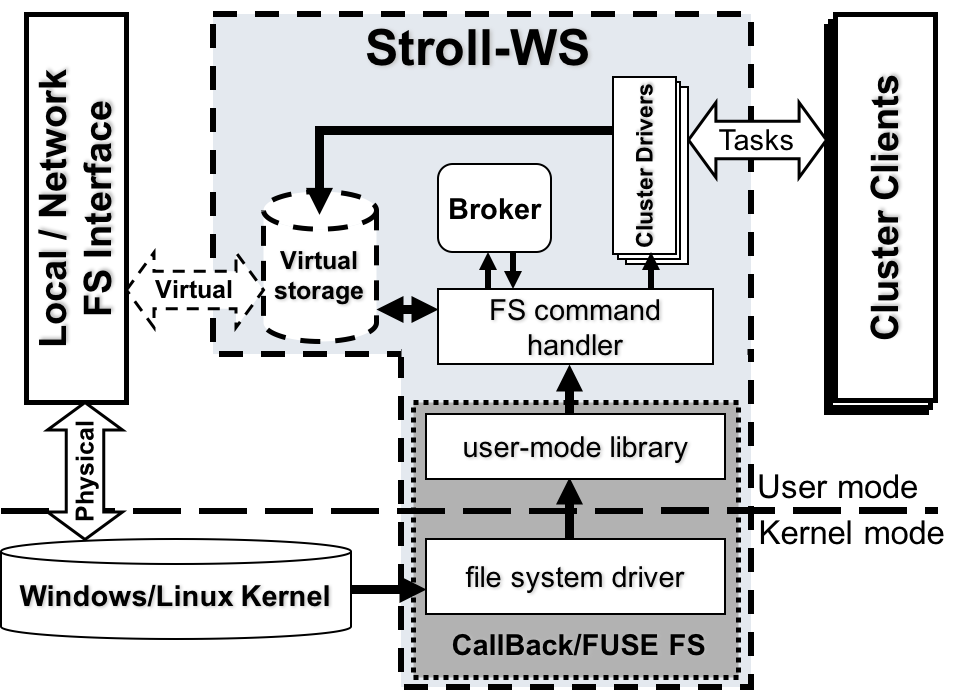
\includegraphics[width=0.9\linewidth]{figures/stroll-ws}                
		\label{fig:stroll-ws}
	}\qquad
	\subfloat[Client-server Architecture]{
		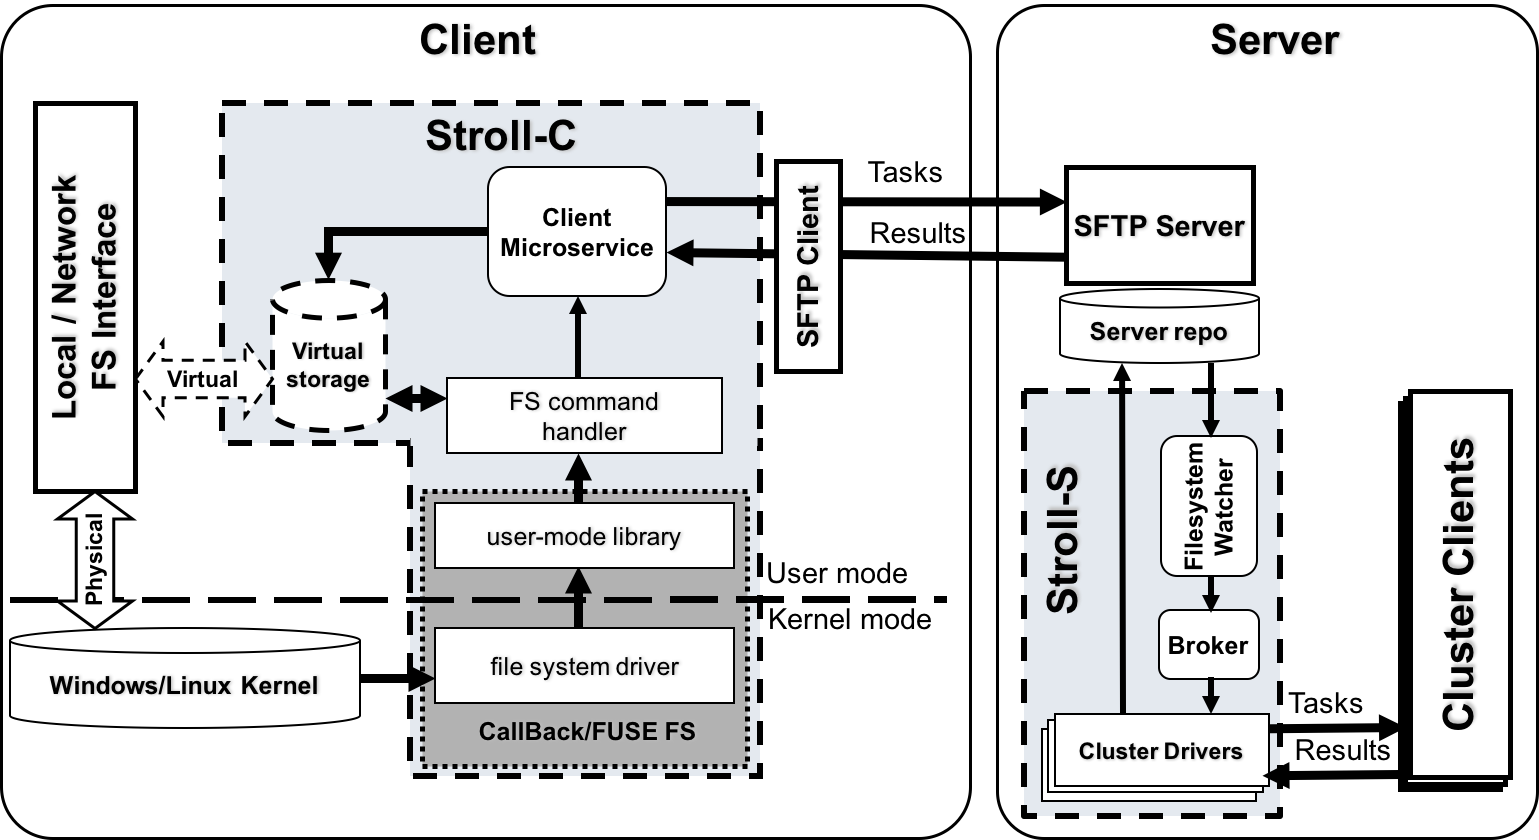
\includegraphics[width=1.0\linewidth]{figures/stroll-cs}                
		\label{fig:stroll-cs}
	}\\
	\caption{\name Architecture}
	\vspace{-.3cm}
	\label{fig:stroll-arch}
\end{figure}

\subsection{\name Task Structure}
\label{sec:task-structure}

In the \name model a cluster job is composed of: the executable, job input files, and the configuration file (e.g. job submission script). Since \name provides an alternate submission and manipulation mechanism based on \fs interface, The submission script is replaced by \name \fs submission and monitoring commands. The following are the general job identity rules:
\begin{itemize}
	\item Each cluster job has a separate directory on \name \fs
	\item The job name is the job directory name
	\item Job names must be unique
\end{itemize}
\figref{fig:job-structure} presents the directory structure of a \name job.

\begin{figure}[htbp]
	\centering
	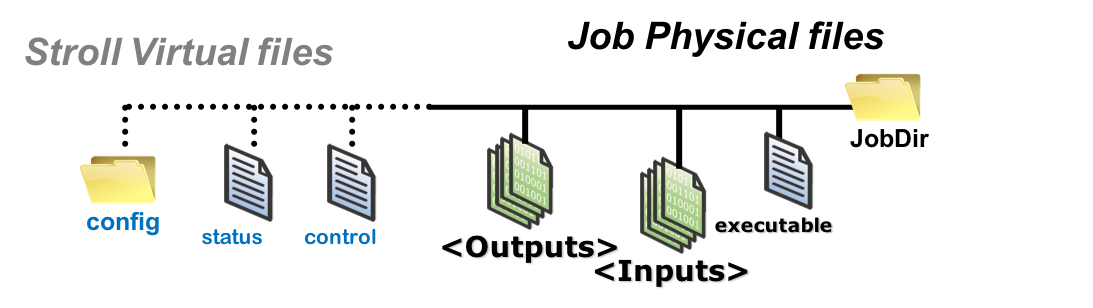
\includegraphics[width=.9\linewidth]{figures/job-structure}                
\caption{\name job directory structure}
\label{fig:job-structure}
\end{figure}

Files in a \name job directory are classified into: i)~\textit{actual job files}, which are the original cluster job files, e.g. the executable and the input files. ii)~\textit{virtual control files}, which are automatically created by \name for the user to configure, monitor and control the job execution and mainly three:
\begin{enumerate}
    \item \textit{status} file, which has only read access and displays the task status in real-time, e.g. state (running, waiting, or halted).
	 \item \textit{control} file, which has only write access and is used to execute task control commands, e.g. submission and forced termination. Three control commands are supported:
	 \begin{itemize}
		\item \textsc{submit}: Submits the job for execution.
		\item \textsc{terminate}: Forces job termination.  
		\item \textsc{restart}: Terminates the job and re-submits it.  
	\end{itemize}
	  \item \textit{config} directory file, is a repository for the job configuration parameters and is composed of a set of virtual files each named as a configuration parameter and contains the value of this particular parameter as text. 

\end{enumerate}
